\documentclass[14pt,a4paper]{article}
\usepackage[14pt]{extsizes}
\usepackage[left=1.5cm, right=1.5cm, top=1.5cm, bottom=1.5cm]{geometry}
\usepackage[utf8]{inputenc}
\usepackage[T2A]{fontenc}
\usepackage[english, russian]{babel}
\usepackage{amsmath,amsfonts,amssymb,amsthm,mathtools} 
\usepackage{amsfonts}
\usepackage{amssymb}
\usepackage{titleps}
\usepackage{hyperref}
\usepackage{float}
\usepackage{graphicx}
\usepackage{multirow}
\usepackage{hhline}
\usepackage{wrapfig}
\usepackage{tikz}
\usepackage{pgfplots}
\usepackage{xcolor}
\usepackage{subfig}
\usepackage{upgreek}

\newcommand{\w}[1]{\text{#1}}
\newcommand{\und}[1]{\underline{#1}}
\newcommand{\img}[3]{
	\begin{figure}[H]
	\begin{center}
	\includegraphics[scale=#2]{#1}
	\end{center}
	\begin{center}
 	\textit{#3}
	\end{center}
	\end{figure}
}
\newcommand{\aw}[1]{
	\begin{center}
	\textit{#1}
	\end{center}
	\n
}
\newcommand{\be}[1]{
	\begin{center}
	\boxed{#1}
	\end{center}
}
\newcommand{\beb}[1]{
	\begin{equation}
	\boxed{#1}
	\end{equation}
}
\newcommand{\eb}[1]{
	\begin{equation}
	#1
	\end{equation}
}
\newcommand{\n}{\hfill \break}
\newcommand{\x}{\cdot}

\begin{document}

\begin{center}
{\large МОСКОВСКИЙ ФИЗИКО-ТЕХНИЧЕСКИЙ ИНСТИТУТ (НАЦИОНАЛЬНЫЙ ИССЛЕДОВАТЕЛЬСКИЙ УНИВЕРСИТЕТ)}
\end{center}
	
\vspace{4.5cm}
{\huge
\begin{center}
{\bf Отчёт о выполнении лабораторной работы 3.1.3}\\	
Измерение магнитного поля Земли		
\end{center}
}
\vspace{2cm}
\begin{flushright}
{\LARGE Автор:\\ Киркича Андрей Александрович \\
\vspace{0.2cm}
Б01-202}
\end{flushright}
\vspace{4cm}
\begin{center}
Долгопрудный, \today
\end{center}

\newpage
\n
	\textbf{Цель работы: }
	исследовать свойства постоянных неодимовых магнитов; измерить с их помощью горизонтальную и вертикальную составляющие индукции магнитного поля Земли и магнитное наклонение.
	\n\n
	\textbf{В работе используются: }
	неодимовые магниты; тонкая нить для изготовления крутильного маятника; медная проволока; электронные весы; секундомер; измеритель магнитной индукции; штангенциркуль; брусок, линейка и штатив из немнагнитных материалов; набор гирь и разновесов.
	\section*{Теоретичские сведения и описание установки}
	Простейший магнитный диполь может быть образован витком с током или постоянным магнитом. По определению, магнитный момент $\overrightarrow{P_m}$ тонкого витка площадью $S$ с током $I$ равен:
$$
\overrightarrow{P_m}=\dfrac{I}{c}\vec{S}=\dfrac{I}{c}S\vec{n},
$$
где $\vec{S}=S\vec{n}$ -- вектор площади круга контура. Если размеры контура с током или магнитной стрелки малы по сравнению расстоянием до диполя, то соответствующий магнитный диполь называют элементарным или точечным.\\
Магнитное поле точечного диполя определяется по формуле, аналогичной формуле для поля
элементарного электрического диполя:
$$
\vec{B}=\dfrac{3(\overrightarrow{P_m} \x \vec{r})\vec{r}}{r^5} - \dfrac{\overrightarrow{P_m}}{r^3}.
$$ 
В магнитном поле с индукцией $B$
на точечный магнитный диполь 
действует механический
момент сил:
$$
\vec{M} = \overrightarrow{P_m}\times \vec{B}.
$$
Под действием вращающего момента $\vec{M}$ виток с током или постоянный магнит поворачивается
так, чтобы его магнитный момент выстроился вдоль вектора индукции магнитного поля. Это —
положение устойчивого равновесия: при отклонении от этого положения возникает механический
момент внешних сил, возвращающий диполь к положению равновесия. В положении, когда $\overrightarrow{P_m}$ и $\vec{B}$
параллельны, но направлены противоположно друг другу, также имеет место равновесие ($M$ = 0),
но такое равновесие неустойчиво: малейшее отклонение от этого положения приведёт к появлению
момента сил, стремящихся отклонить диполь ещё дальше от начального положения.\n\n
Магнитный диполь в магнитном поле обладает энергией:
$$
W = -(\overrightarrow{P_m} \x \vec{B}).
$$
В неоднородном поле на точечный магнитный диполь, кроме момента сил, действует ещё и сила:
$$
\vec{F}=(\overrightarrow{P_m} \x \vec{\triangledown})\vec{B}.
$$
Используя формулы для момента силы, силы и энергии, не сложно выяснить, как ведёт себя
свободный магнитный диполь в неоднородном магнитном поле: он выстраивается вдоль силовых
линий магнитного поля и, кроме того, под действием результирующей силы, возникающей из-за
неоднородности поля, втягивается в область более сильного магнитного поля, т.е. в область, где он
обладает меньшей энергией.\n\n
Зная магнитные моменты $P_1 = P_2 = P_m$ двух небольших постоянных магнитов, можно рассчитать силу
их взаимодействия:
$$
F = P_m \dfrac{\partial B}{\partial r}=-6\dfrac{P_m^2}{r^4}.
$$
	В настоящей работе используются неодимовые магниты шарообразной формы.
Для нас важно то, что:\n\n
1) Шары намагничены однородно;\\
2) Вещество, из которого изготовлены магниты, является магнитожёстким материалом.\n\n
Полный магнитный момент $\overrightarrow{P_m}$
постоянного магнита определяется намагниченностью $\overrightarrow{p_m}$
вещества, из которого он изготовлен. По определению, намагниченность – это магнитный момент единицы объёма. Для однородно намагниченного шара намагниченность равна:
$$
\overrightarrow{p_m}=\dfrac{\overrightarrow{P_m}}{V}.
$$
Намагниченность — важная характеристика вещества постоянных магнитов, определяющая, в
частности, величину остаточной магнитной индукции $B_r = 4\pi p_m$. Индукция магнитного поля $\overrightarrow{B_p}$
на полюсах однородно намагниченного шара связана с величиной намагниченности и остаточной магнитной индукцией формулами
$$
\overrightarrow{B_p}=\dfrac{8\pi}{3}\overrightarrow{p_m}=\dfrac{2}{3}\overrightarrow{B_r}.
$$
\subsection*{Определение величины магнитного момента магнитных шариков}
\paragraph*{Метод А}\n
Величину магнитного момента одинаковых шариков
можно рассчитать, зная их массу $m$ и определив максимальное расстояние $r_{max}$, на котором они ещё удерживают друг
друга в поле тяжести. При максимальном расстоянии сила тяжести шариков равна силе их магнитного притяжения:
\begin{center}
$\dfrac{6P_m^2}{r_{max}^4}=mg\Rightarrow$ \fbox{$P_m = \sqrt{\dfrac{mgr_{max}^4}{6}}$} .
\end{center}
\paragraph*{Метод Б}\n
Если сила сцепления двух одинаковых шаров диаметром $d$ c магнитными моментами $P_m$ равна
$$
F_0 = \dfrac{6P_m^2}{d^4},
$$
то минимальный вес цепочки, при которой она оторвётся от верхнего шарика равен: $F \approx 1.08 F_0$. Тогда
\begin{center}
\fbox{$P_m = \sqrt{\dfrac{Fd^4}{6.48}}$} .
\end{center}
\subsection*{Определение величины магнитного поля Земли}
\paragraph*{Горизонтальная составляющая}
\begin{wrapfigure}{R}{3.5cm}
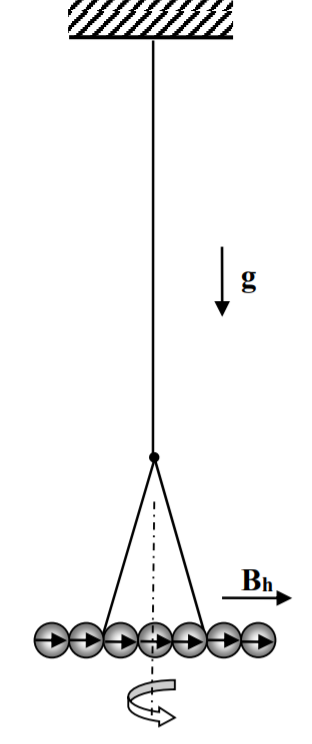
\includegraphics[scale=0.5]{1.png}
\vspace{-40pt}
\end{wrapfigure}\n
Магнитная <<стрелка>> образована из $n$ сцепленных друг с другом противоположными полюсами шариков и с помощью $\Lambda$-образного подвеса подвешена в горизонтальном положении. При отклонении «стрелки» на угол $\theta$ от равновесного положения в горизонтальной плоскости возникают крутильные колебания вокруг вертикальной оси, проходящей через середину стрелки. При малых амплитудах уравнение колебаний
стрелки имеет вид:
$$
I_n \dfrac{d^2 \theta}{dt^2} + P_0 B_h \theta = 0,
$$
\begin{wrapfigure}{L}{6cm}
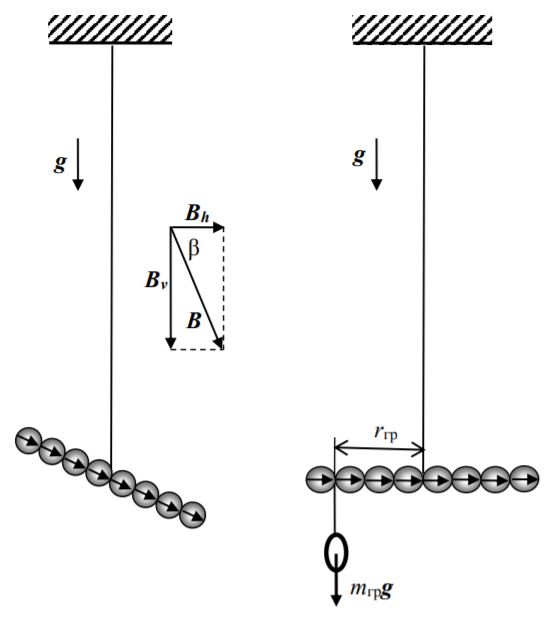
\includegraphics[scale=0.5]{2.png}
\vspace{-10pt}
\end{wrapfigure}
где $P_0$ -- магнитный момент стрелки, $B_h$ -- горизонтальная составляющая магнитного поля Земли, $I_n \approx \dfrac{1}{12}n^3 m d^3$.
\n\n
Тогда период колебаний $T = kn$, где $k = \pi \sqrt{\dfrac{md^2}{3P_m B_h}}$. Измерив зависимость $T=T(n)$, можно найти $B_h$:
\begin{center}
\fbox{$B_h = \dfrac{\pi^2 m d^2}{3k^2P_m}$} .
\end{center}

\paragraph*{Вертикальная составляющая}
\n
Магнитная «стрелка», составленная из чётного числа
шариков и подвешенная на тонкой нити за середину, расположится не горизонтально, а под некоторым, отличным от нуля, углом к горизонту. Это связано с тем, что вектор $\vec{B}$ индукции магнитного поля Земли в общем случае не горизонтален, а образует с горизонтом
угол $\beta$, зависящим от географической широты $\varphi$
места, где проводится опыт. Величина угла $\beta$
называется магнитным наклонением.\\
С помощью небольшого дополнительного грузика «стрелку» можно «выровнять». Момент $M$ силы тяжести уравновешивающего груза пропорционален числу $n$ шариков, образующих магнитную «стрелку» $M(n) = An, A=P_m B_v$. Перепишем последнюю формулу в виде:
\begin{center}
\fbox{$B_v = \dfrac{A}{P_m}$} .
\end{center}
В дальнейшем мы будем использовать эту формулу для расчёта вертикальной составляющей магнитного поля.

\section*{Ход работы}
Определим параметры шариков: масса 12 штук $m_{12} = 10,139 \pm 0,001\text{ г}$, тогда масса одного $m = (8,449 \pm 0,001) \cdot 10^{-1}~\text{г}$, диаметр $d = 5,64 \pm 0,01~\text{мм}$.\\
Для измерения $r_{max}$ поместим шарики по разные стороны бумажных листов так, чтобы они всё ещё притягивались, и будем подкладывать листы бумаги между ними до тех пор, пока сила тяжести не пересилит силу притяжения. Измеренный $r_{max} = 1,95 \pm 0,05~\text{см}$. Тогда: 
\n\n
$P_m = 44,7 \pm 0,3 \frac{\text{эрг}}{\text{Гс}}, \quad p_m = 475 \pm 11 \text{Гс}, \quad B_p = 4,0 \pm 0,1 \text{кГс}, \quad B_r = 5970 \pm 140 \text{Гс}$.
\n\n
Измерения датчиком Холла: $B_p = 386 \pm 1\text{мТ}=3,86 \pm 0,01\text{кГс}.$
За итоговый магнитный момент возьмём $P_m = 44,7 \pm 0,3\text{эрг/Гс}$, так как показания датчика близки к нему.
Соберём установку для измерения горизонтальной составляющей магнитного поля Земли. Перед непосредственным измерение проверим, можно ли пренебречь упругостью нити при измерении периода колебаний. Для этого сделаем из шариков кольцо, чтобы магнитный момент был нулевым, и посмотрим на его период колебаний $T = 131 \pm 1~\text{с}$. Такой большой период колебаний указывает на то, что упругостью можно пренебречь.
\begin{table}[h]
\centering
\begin{tabular}{|r|r|r|r|r|r|r|r|r|r|r|}
\hline
$n$ & 12    & 11    & 10    & 9     & 8     & 7     & 6     & 5     & 4     & 3    \\ \hline
$T$, с & 3.4 & 3.1 & 2.8 & 2.6 & 2.3 & 1.9 & 1.7 & 1.4 & 1.1 & 0.8 \\ \hline
\end{tabular}
\end{table}
%\begin{center}
%\resizebox{400pt}{!}{
%\begin{tikzpicture}[scale=1]
%    	\begin{axis}[
%    		axis lines = left,
%        	xlabel = {$n$},
%        	ylabel = {$T$, с},
%        	ylabel style={scale=1},
%        	xlabel style={scale=1},
%        	%xmin=0, xmax=9,
%        	legend style={at={(0.03,-0.4)},anchor=west}
%    		]
%    		\addplot +[only marks]  plot[
%			error bars/.cd,
%			x dir = both,
%			x fixed relative = 0.01,
%			y dir = both,
%			y fixed relative=0.01,
%		    ]
%		    table[x=n, y=T]{Plot1.txt};
%		    \addplot[domain=0:12]{0.27461 * x + 0.077509};
%    	\end{axis}
%    \end{tikzpicture}
%    }
%\end{center}
%Полученный коэффциент наклона $k= 0.28 \pm 0.01~\text{с}$. Тогда 
Получаем:
\begin{center}
\fbox{$B_h = 0.26 \pm 0.01~\text{Гс}$} .
\end{center}
	Уравновесим магнитные <<стрелки>>, измерив $M(n)$:
\n\n
\begin{minipage}{0.4\textwidth}
\begin{tabular}{|c|c|c|c|}
\hline
n  & k & m, г  & M, дин $\x$ см \\ \hline
12 & 5 & 0.174 & 481 \\ \hline
10 & 4 & 0.236 & 522 \\ \hline
8  & 3 & 0.237 & 393 \\ \hline
6  & 2 & 0.296 & 327 \\ \hline
4  & 1 & 0.434 & 240 \\ \hline
\end{tabular}
\end{minipage}
\begin{minipage}{0.2\textwidth}
\begin{tikzpicture}[scale=1]
    	\begin{axis}[
    		axis lines = left,
        	xlabel = {$n$},
        	ylabel = {$M$, дин $\x$ см},
        	ylabel style={scale=1},
        	xlabel style={scale=1},
        	%xmin=0, xmax=9,
        	legend style={at={(0.03,-0.4)},anchor=west}
    		]
    		\addplot +[only marks]  plot[
			error bars/.cd,
			x dir = both,
			x fixed relative = 0.01,
			y dir = both,
			y fixed relative=0.01,
		    ]
		    table[x=n, y=L, col sep=semicolon]{Plot2.txt};
		    \addplot[domain=0:12]{33.85 * x + 121.8};
    	\end{axis}
    \end{tikzpicture}
\end{minipage}
\n\n
Тогда:
\begin{center}
\fbox{$B_v = 0.76 \pm 0.04~\text{Гс}$} .
\end{center} 
	\section*{Заключение}
	Итоговая индукция магинтного поля Земли $B = \sqrt{B_v^2 + B_h^2} = 0.80 \pm 0.05 \ \text{Гс}$. Это больше, чем табличные значения, которые находятся в диапазоне $0.60 - 0.65$ Гс. Причиной отклонения может быть работа электронных устройств (таких как мобильные телефоны или нотбуки) около экспериментальной установки, которая ведёт к искажению магнитного поля.
Магнитное наклонение $\beta= \text{arctg}~\dfrac{B_v}{B_h}=71^\circ\pm 4^\circ$.
\end{document}